\documentclass[10pt]{article}
\usepackage[utf8]{inputenc}
%\usepackage[T1]{fontenc}
\usepackage{tgbonum}
\usepackage[english]{babel}
\usepackage{graphicx}
\usepackage{amsmath}
\usepackage{amssymb}
\usepackage{hyperref}
\usepackage{epsf}
\usepackage{float}
\usepackage{mathpazo}
\usepackage{pifont}
\usepackage
[
a4paper,% other options: a3paper, a5paper, etc
left=2.2cm,
right=2.2cm,
top=2cm,
bottom=2cm,
]{geometry}
%\geometry{hmargin=3.5cm, vmargin=2.5cm}
\usepackage{fancyhdr}
\pagestyle{fancy}
\fancyhf{}
\rfoot{\thepage}
\renewcommand{\headrulewidth}{0pt}
\usepackage{color}
\usepackage{graphicx}
\usepackage{wrapfig}
\usepackage{graphicx}
\usepackage{multicol}
\usepackage{enumitem}
\usepackage{xcolor}
\usepackage{framed}
\usepackage{bm}
\definecolor{shadecolor}{RGB}{139, 231, 3}
\usepackage{epigraph}

\usepackage{tcolorbox}
\definecolor{mycolor}{rgb}{0.122, 0.435, 0.698}

\newtcbox{\mb}{nobeforeafter,colframe=mycolor,colback=mycolor!10!white,boxrule=0.5pt,arc=4pt,
  boxsep=0pt,left=6pt,right=6pt,top=3pt,bottom=3pt,tcbox raise base}

\usepackage{eso-pic}
\newcommand\BackgroundPic{%
\put(-0,-150){%
\parbox[b][\paperheight]{\paperwidth}{%
\vfill
\centering
\includegraphics[width=\paperwidth,%
keepaspectratio]{DWGs/foret-de-soignes.jpg}%
\vfill
}}}

\usepackage[T1]{fontenc}

\usepackage{anyfontsize}
\usepackage{t1enc}
\newcommand{\heart}{\ensuremath\varheartsuit}
\usepackage{tikz}
\usetikzlibrary{positioning}
\usepackage{charter}

\begin{document}

% TITLE PAGE ====================================================

\begin{titlepage}
\AddToShipoutPicture*{\BackgroundPic}
\ \\[4cm]
{\sffamily \color{white}
\begin{center}
\fontsize{34}{10}\selectfont \fontfamily{ppl}\selectfont Computational examples 

\fontsize{20}{10}\selectfont \fontfamily{ppl}\selectfont in 

\,\,\,

\fontsize{40}{10}\selectfont \fontfamily{ppl}\selectfont  transport phenomena

\,\,\,

\fontsize{25}{10} \selectfont \fontfamily{augie}\selectfont with Python

\end{center}
}
\vfill
{\fontsize{20}{20}\color{white}\sffamily Science Docs \hfill\color{white} Kamila Zdybał}

{\fontsize{10}{10}\color{white}\sffamily PDFs for explorers and experimenters}
\end{titlepage}


% EX LIBRIS PAGE ================================================

\thispagestyle{empty}
\begin{center}

This document was prepared as part of the course \textit{The Basics of Transport Phenomena} from Delft University of Technology, available on edX.org as DelftX: TP101x.

This material was created by or adapted from material posted on the DelftX website, delftx.tudelft.nl, and created by TU Delft faculty members Robert Mudde, Professor of Multiphase Flow at the Dept. of Chemical Engineering and Peter Hamersma, Associate Professor at the Dept. of Chemical Engineering, 2015. DelftX is not responsible for any changes made to the original materials posted on its website and any such changes are the sole responsibility of Kamila Zdybał.

The course materials by Delft University of Technology are subjected to copyright and are licensed under a Creative Commons Attribution-NonCommercial-ShareAlike 4.0 International License.

https://creativecommons.org/licenses/by-nc-sa/4.0/

\vspace*{6cm}


\setlength{\parskip}{0.0em}
\setlength{\parindent}{0cm}

Copyright \textcopyright \, K. Zdybał, 2018

For more projects similar to this one

visit me on GitHub: \verb|@camillejr|

\verb|camillejr.github.io/science-docs/|

To contact me personally drop me a line at:

\verb|kamilazdybal@gmail.com|

\vspace*{1cm}

Cover picture: \textit{Forêt de Soignes, Belgium}

Photo taken on: 16 Jan 2017

Copyright \textcopyright \, K. Zdybał, 2017

\vspace*{6cm}

\verb|Computational examples in transport phenomena with Python|

Typeset with \LaTeX

\vspace*{2cm}

\noindent This work is licensed under the Creative Commons

Attribution-NonCommercial-ShareAlike 4.0 International 

(CC BY-NC-SA
4.0) license.

\end{center}
\setlength{\parskip}{0.6em}
\setlength{\parindent}{0.5cm}

\newpage

\tableofcontents

\newpage

\setlength{\parskip}{0.6em}
\setlength{\parindent}{0cm}


\,\,\,

\normalsize

\section{General remarks on transport of physical properties}

The general equation for the transport of a property $\psi$ within a control volume is:

\begin{equation}
\frac{d \psi}{dt} = \Psi_{in} - \Psi_{out} + \Psi_{production} - \Psi_{consumption}
\end{equation}

where $\frac{d \psi}{dt} = \dot{\psi}$ is the flux of the property $\psi$.

\newpage

\section{Steady-state conduction in a lengthwise-insulated rod with internal heat production}

We derive a one-dimensional temperature distribution function $T(x)$ for a steady-state heat conduction in a straight rod of length $L$. We assume that the internal heat production $Q_p$ in units of $W/m^3$ is present at every point inside the rod volume. This may for instance simulate heating up of a wire due to electrical current. The rod is perfectly insulated along its length and it loses heat only through its endpoints which in a steady-state case are kept at a fixed temperature $T_0$.

\begin{figure}[H]
\centering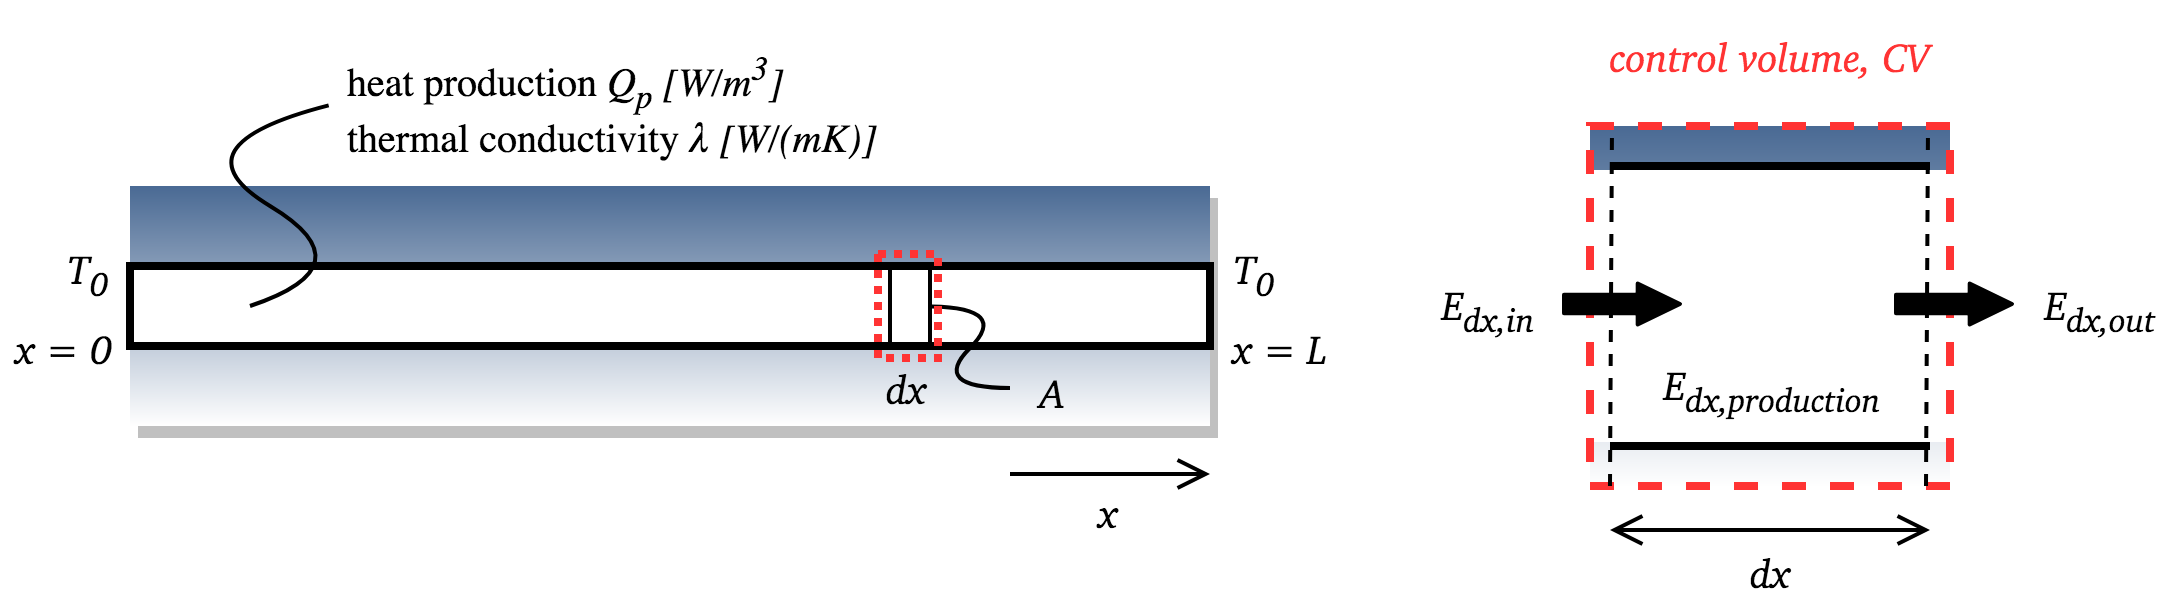
\includegraphics[width=16cm]{DWGs/cond-rod.png}
\caption{Conduction in a rod with internal heat production.}
\label{fig:conduction}
\end{figure}

We will take for the control volume a slice $dx$ from the rod.  The energy balance for the rod element $dx$:

\begin{equation}
\frac{dE_{dx}}{dt} = E_{dx, in} - E_{dx, out} + E_{dx, production}
\end{equation}

Note here that $E_{dx, in}$, $E_{dx, out}$ and $E_{dx, production}$ are energies per unit time and so have the units of $W$.

The heat flux $\phi$ which has units of $W$ can be modeled using the Fourier's law for one-dimensional heat conduction:

\begin{equation}
\phi = \lambda A \Big(- \frac{dT}{dx} \Big)
\label{eq:fourier}
\end{equation}

where $\lambda$ is the thermal conductivity and is a property of the material, $A$ is the rod's cross-sectional area and $\frac{dT}{dx}$ is a temperature gradient which plays a role of the driving force for thermal energy transport.

Hence:

\begin{equation}
E_{dx, in} = \lambda A \Big(- \frac{dT}{dx} \Big)_x
\end{equation}

\begin{equation}
E_{dx, out} = \lambda A \Big(- \frac{dT}{dx} \Big)_{x + dx}
\end{equation}

The energy per unit time coming from the heat production can be written as $Q_p$ multiplied by the volume of the slice $dx$:

\begin{equation}
E_{dx, production} = Q_p A dx
\end{equation}

In the steady-state $\frac{dE}{dt} = 0$ and the energy balance becomes:

\begin{equation}
\lambda A \Big(- \frac{dT}{dx} \Big)_x - \lambda A \Big(- \frac{dT}{dx} \Big)_{x + dx} + Q_p A dx = 0
\end{equation}

Simplifying the above energy balance we get:

\begin{equation*}
\frac{\Big(\frac{dT}{dx} \Big)_{x + dx} - \Big(\frac{dT}{dx} \Big)_x  }{dx} = - \frac{Q_p}{\lambda}
\end{equation*}

It is interesting to note here that we have lost the dependence on the cross-sectional surface area of the rod.

If we now substitute some function $f(x) = \frac{dT}{dx}$ we notice that we have:

\begin{equation*}
\frac{f(x + dx) - f(x)}{dx} = - \frac{Q_p}{\lambda}
\end{equation*}

in other words:

\begin{equation}
\frac{df(x)}{dx} = - \frac{Q_p}{\lambda}
\end{equation}

With the above substitution, the differential equation that we are about to solve becomes:

\begin{equation}
\frac{d^2T}{dx^2} = - \frac{Q_p}{\lambda}
\end{equation}

Applying the boundary conditions from both ends of the rod, the solution to the above differential equation is:

\begin{equation}
T(x) = - \frac{Q_p}{2 \lambda} (x^2 - Lx) + T_0
\label{eq:solution}
\end{equation}

\subsection{Final remarks}

Note that even though the heat flow was assumed to be one-dimensional in this exercise, it does not mean that the geometry of the problem needs to be one-dimensional. In fact, we assumed the rod to be a three-dimensional object having length and a cross-sectional area. Rather, the one-dimensionality of the problem means that it is practical to assume only one of the three directions as an important direction for heat transport. Since the rod was perfectly insulated along its length, the temperature gradient along directions perpendicular to the $x$-axis is zero.

\subsection{Computational example}

As a computational example we will draw the graph of the temperature distribution in a copper rod $200 m$ long. We assume that the thermal conductivity for this rod is $400 \frac{W}{m \cdot K}$. The internal heat production in the entire rod is $20 W$.

\begin{figure}[H]
\centering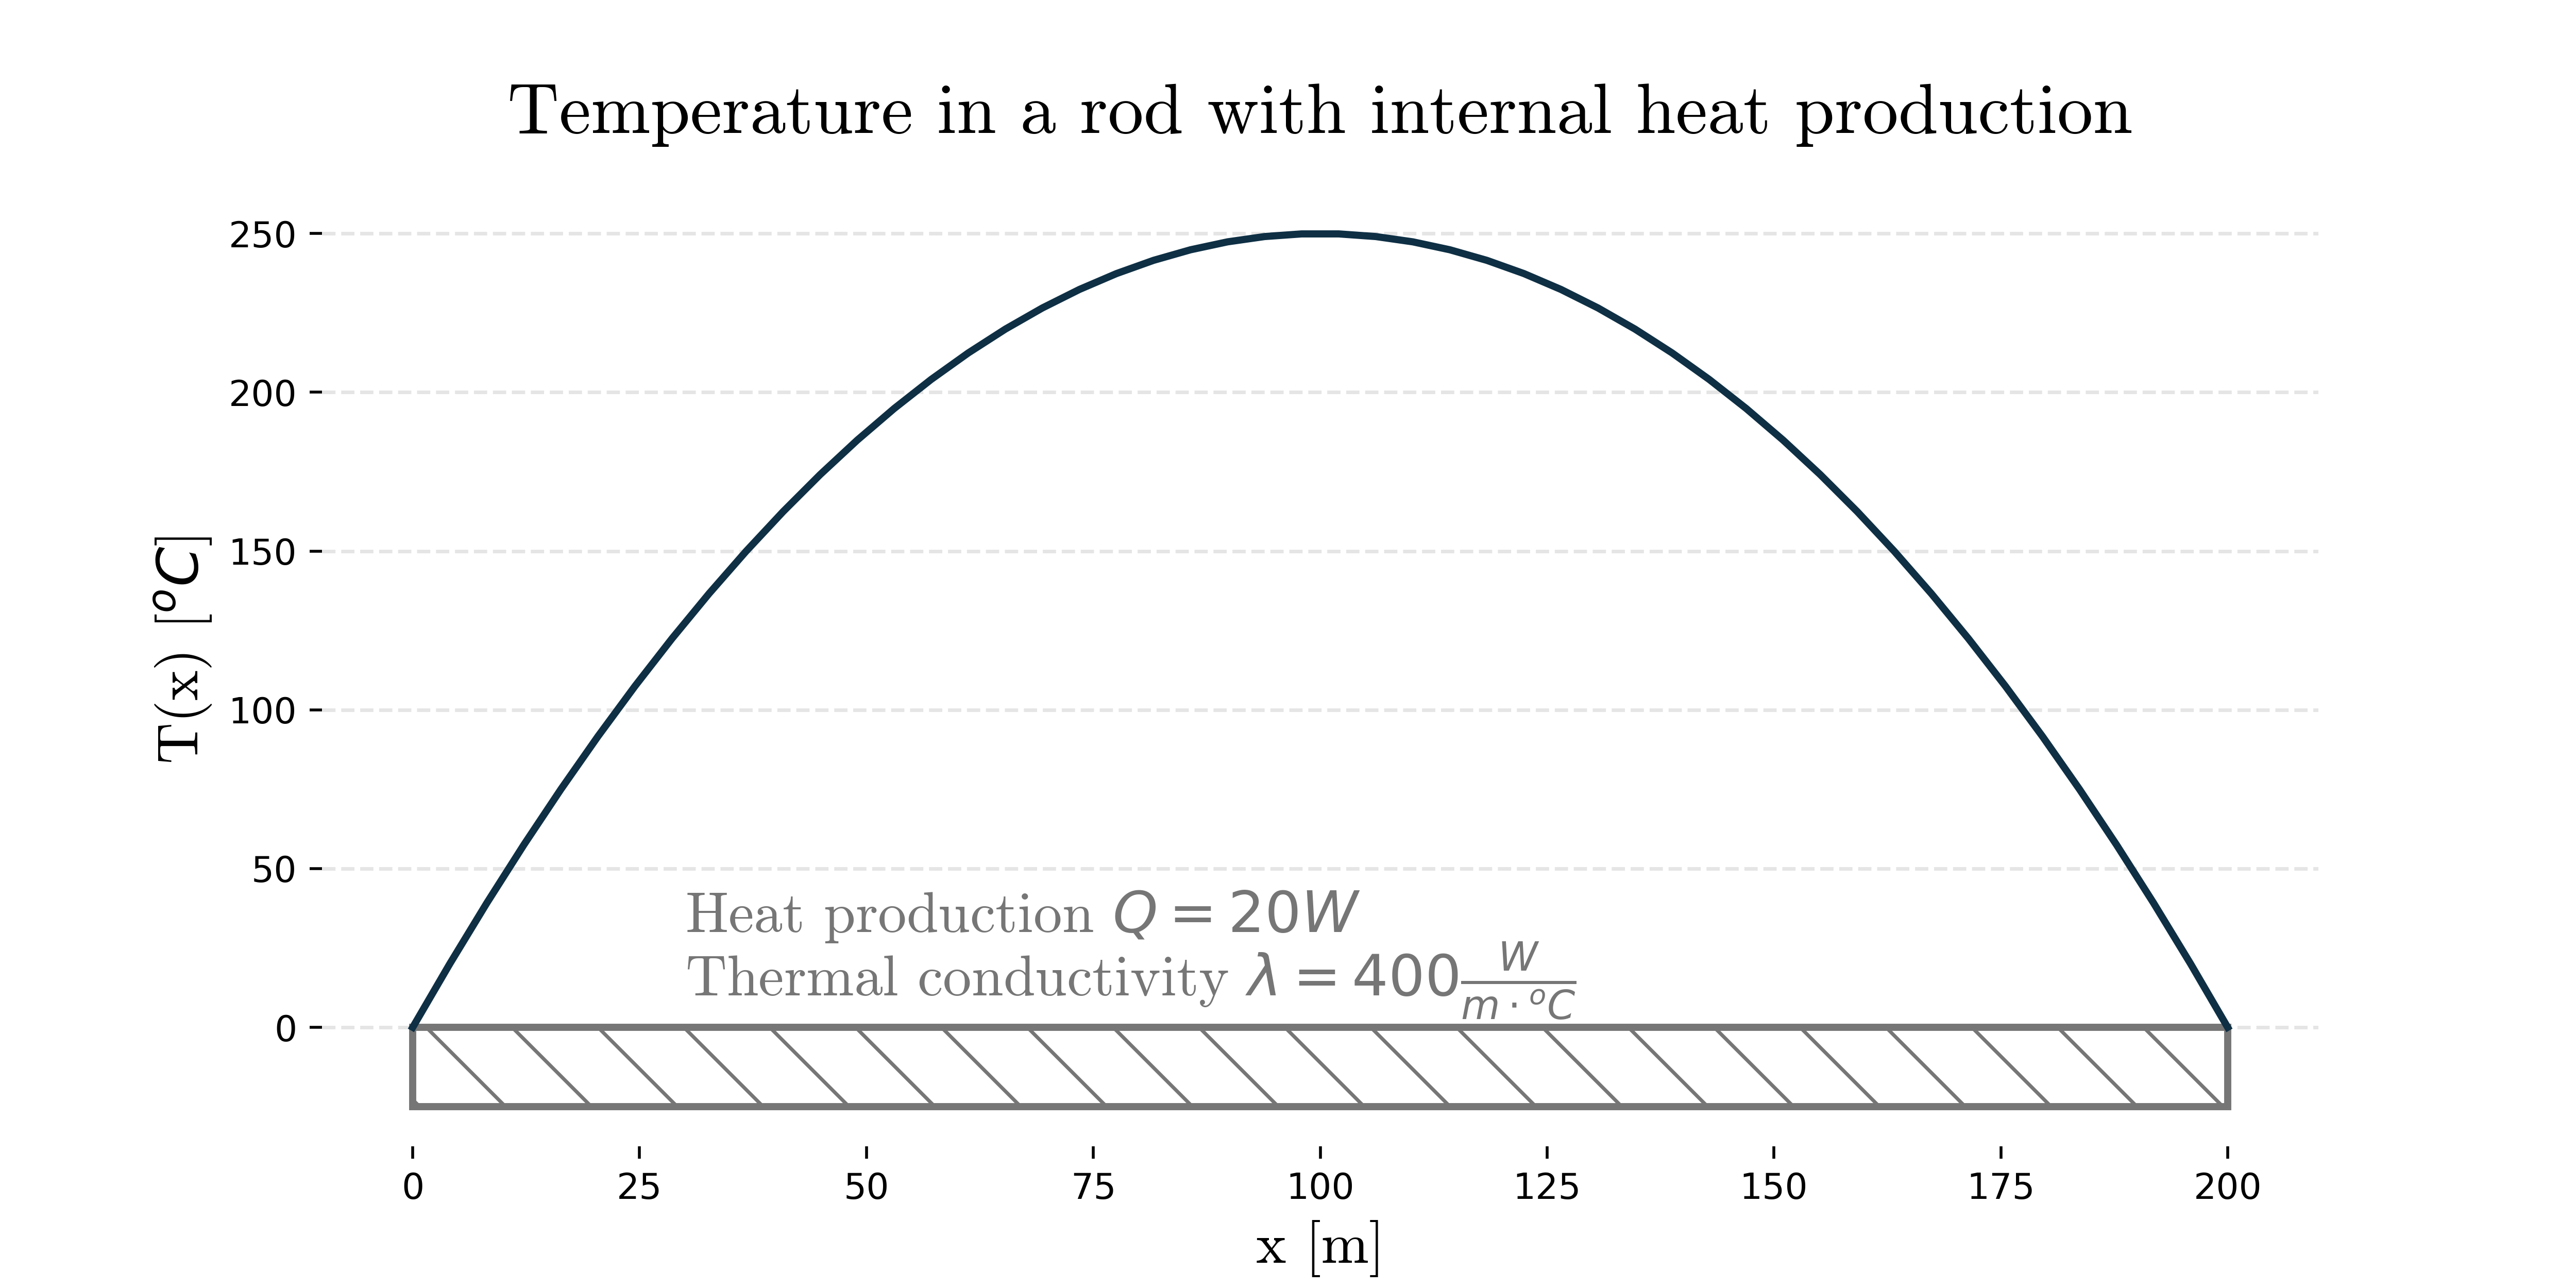
\includegraphics[width=16cm]{Code/conduction-rod.png}
\caption{Temperature distribution in a rod with internal heat production of $20 W$.}
\label{fig:python_graph}
\end{figure}

\newpage

\section{Laminar flows of Newtonian fluids}

\newpage

\section{Lumped system analysis of a steel plate}



\newpage

\section{Evaporating sphere}

\begin{figure}[H]
\centering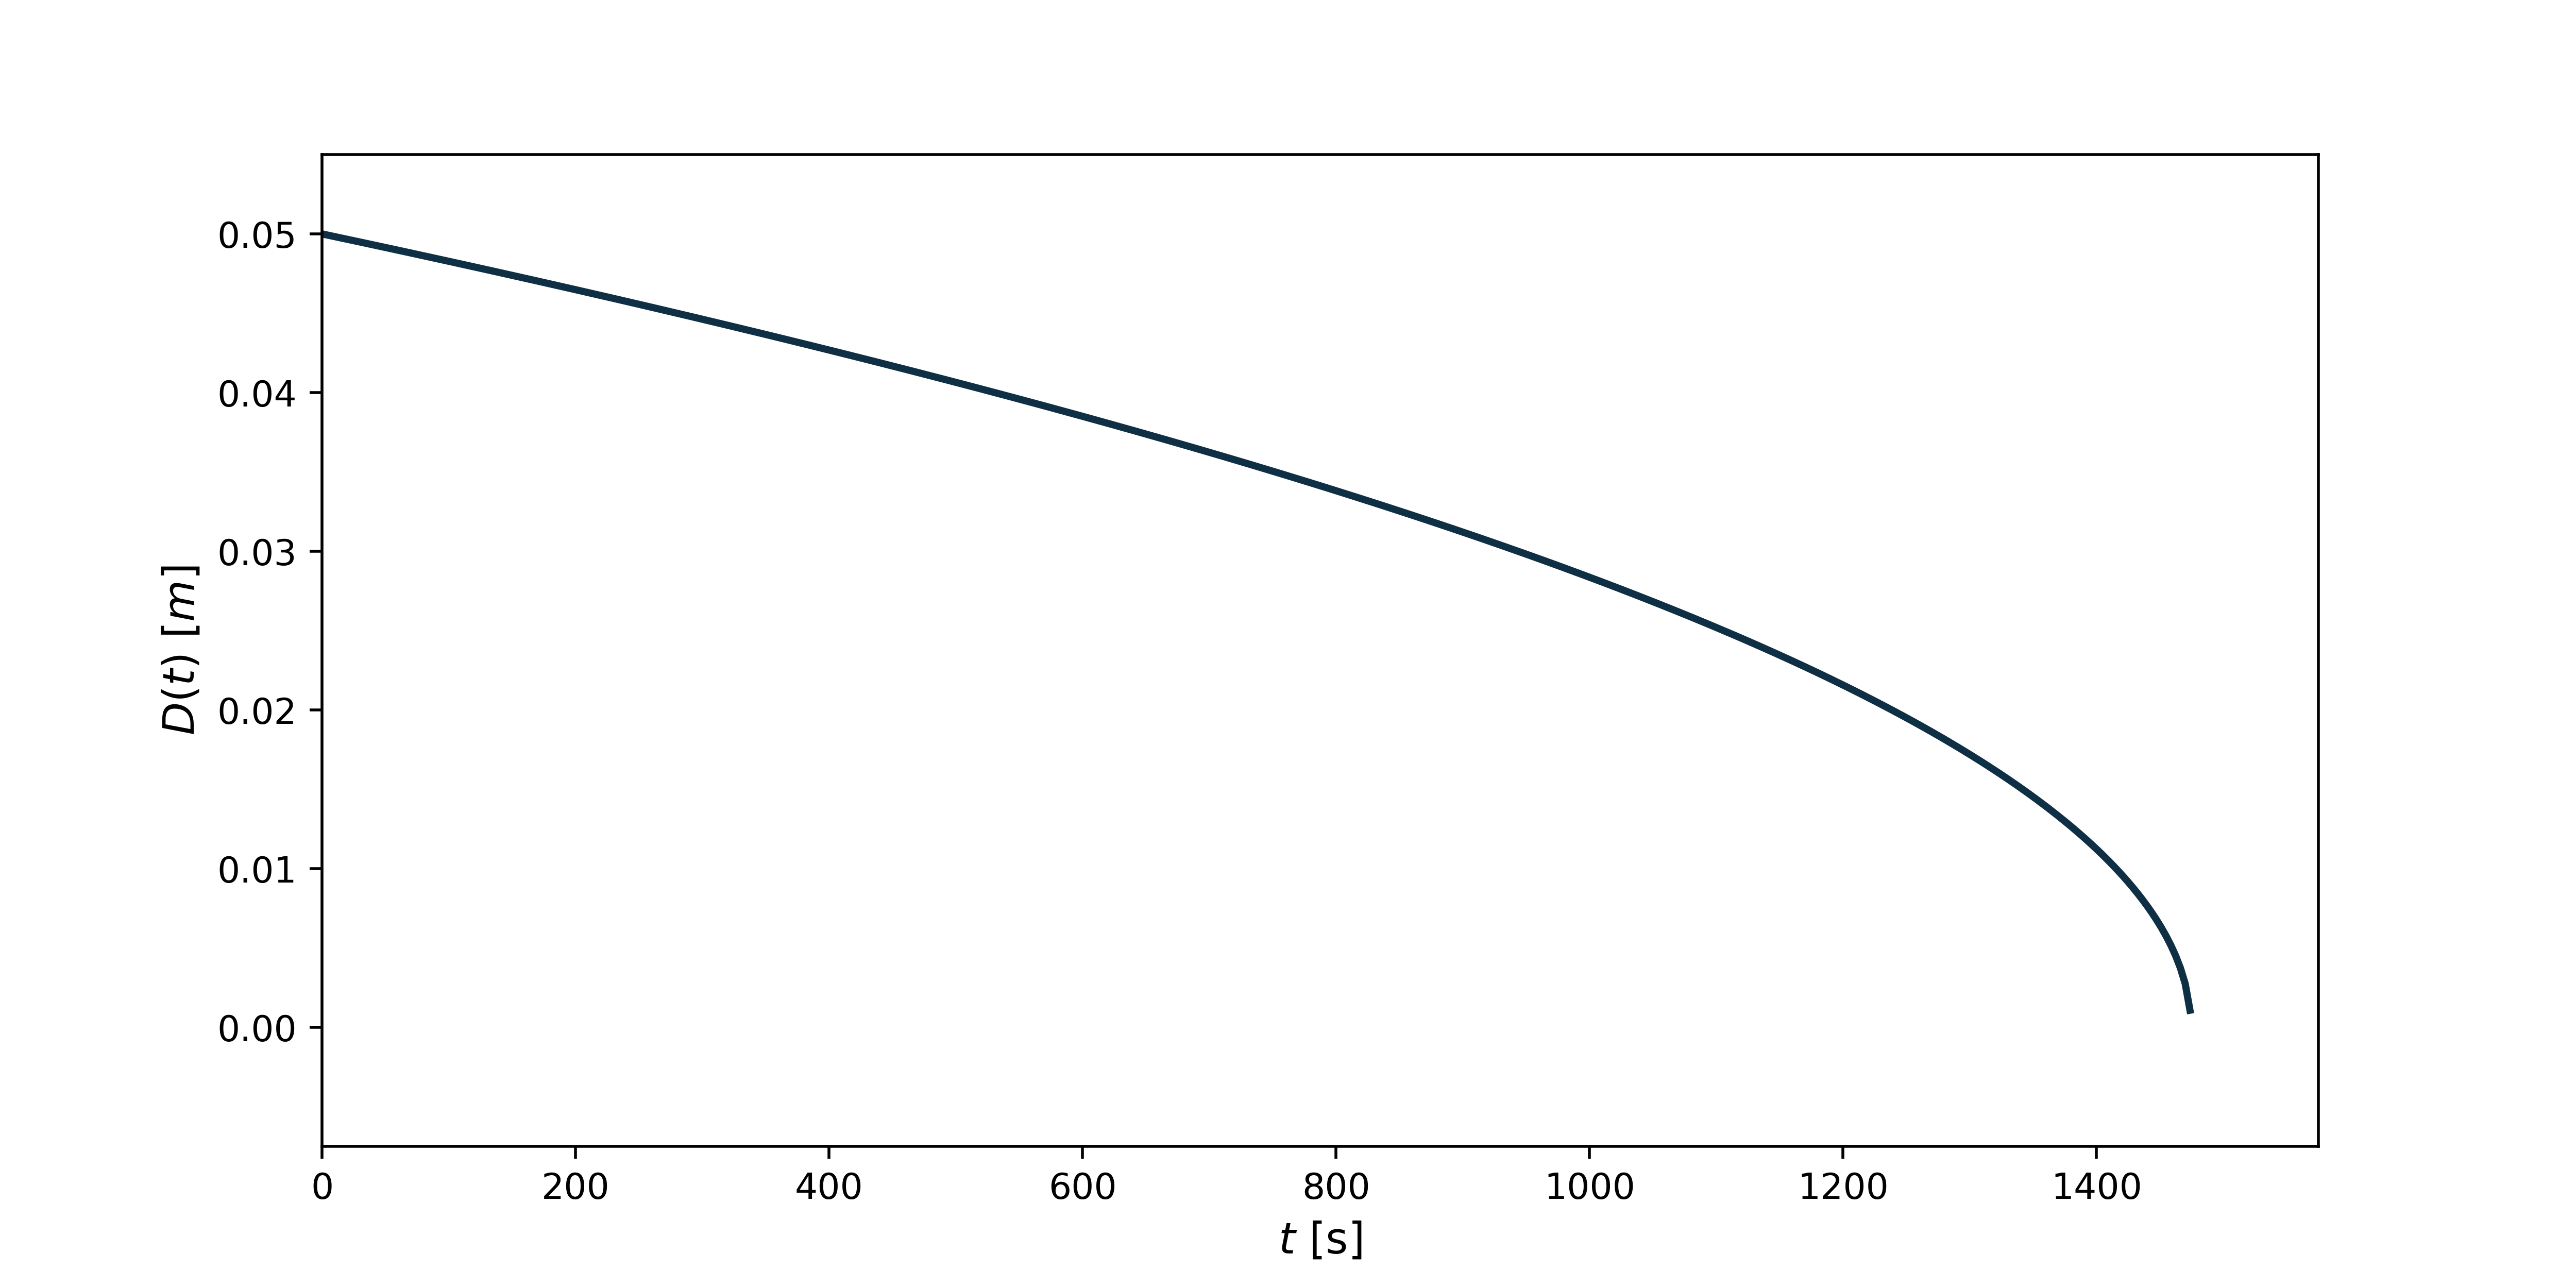
\includegraphics[width=16cm]{Code/evaporating-sphere.png}
\caption{Evaporating sphere diameter history.}
\label{fig:stefan-problem}
\end{figure}

\newpage

\section{One-dimensional binary diffusion}



\newpage

\section{The Stefan problem}

\begin{figure}[H]
\centering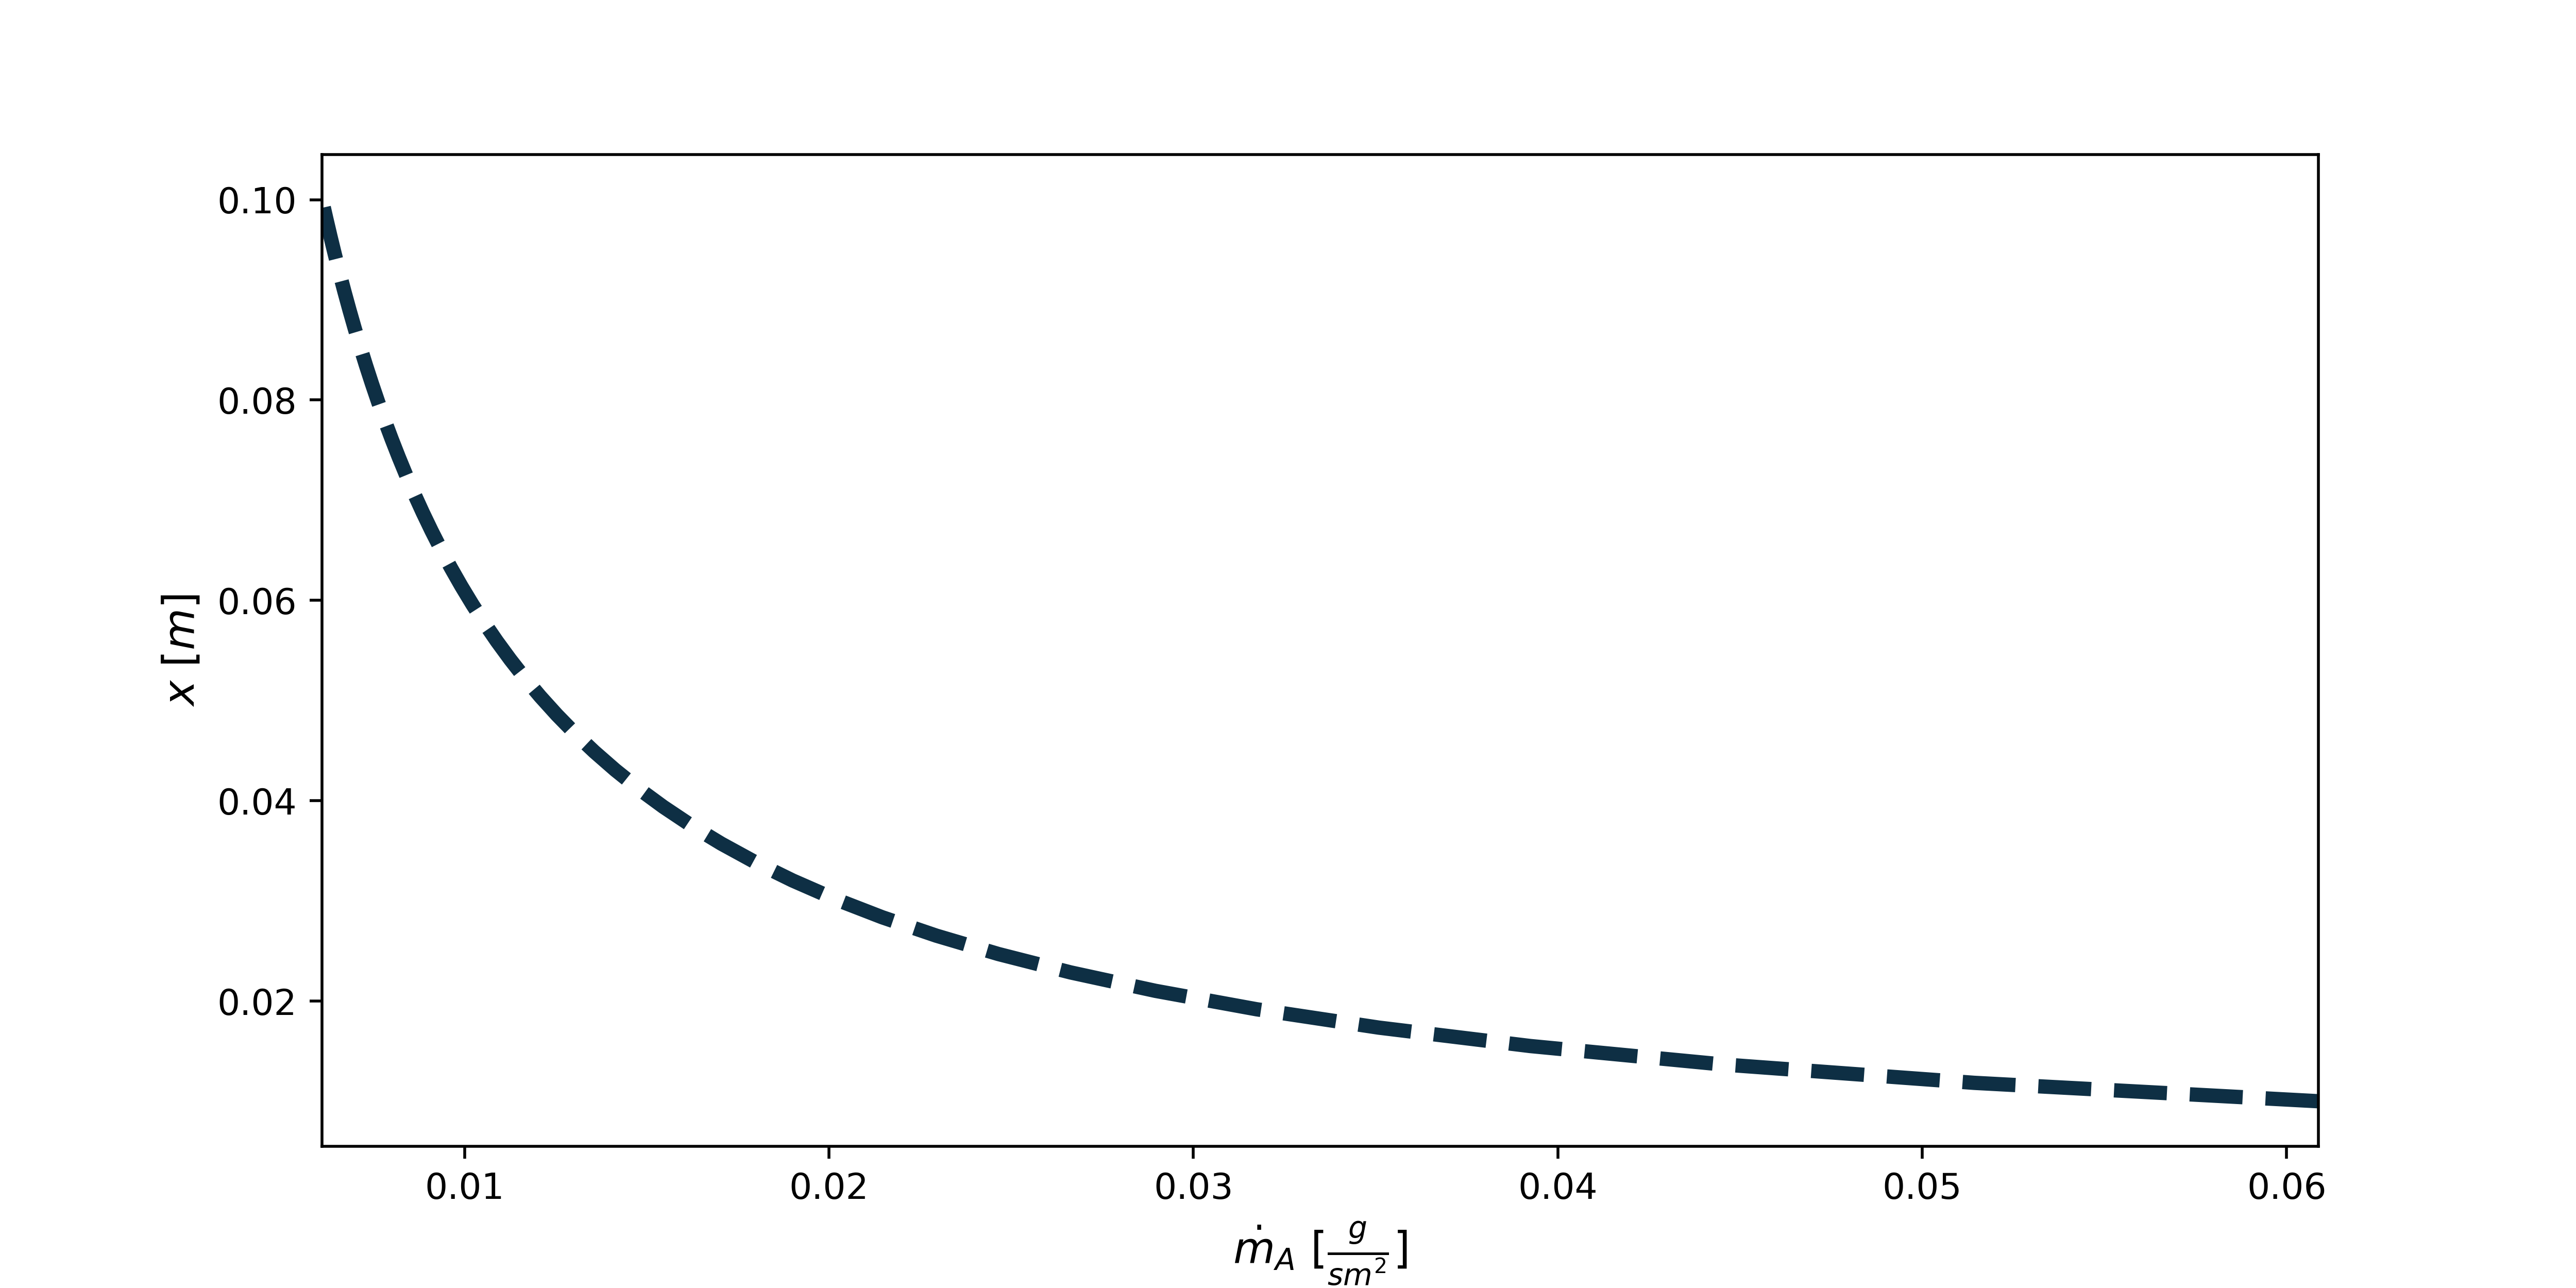
\includegraphics[width=16cm]{Code/stefan-problem.png}
\caption{Stefan problem for water evaporating from the 0.1m tube.}
\label{fig:stefan-problem}
\end{figure}




\end{document}